
\begin{figure}
   \centering
   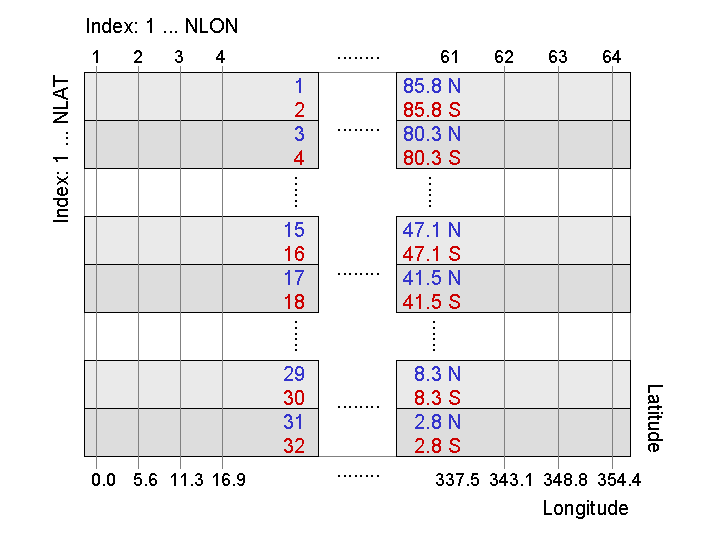
\includegraphics[width=14cm]{Pics/PUMA_alternate_grid.png}
   \caption[]{PUMA T21 horizontal grid sorted by index}
   \label{pumat21igrid}
\end{figure}

PUMA uses internally (other than the Planet Simulator and PUMA version 15) an alternating Gaussian grid.
This feature is unimportant for users, who don't change source code - the output file
will still contain the usual Gaussian grid with the latitude index running from the most Northern latitude
to the most Southern one. But for those, who fiddle around with the code or want to implement additional
arrays it is important to understand the internal structure.

The alternating grid was introduced for two reasons:

1) The number of values for Legendre polynomials could be reduced by a factor of two, because 
pairs of Northern and Southern latitudes with the same absolute value can be processed
simultaneously. This is especially useful for very high resolution runs.
E.g. a PUMA T1365 needs now ca. 45 GByte memory.

2) The Legendre transformation was recoded to use symmetric and antisymmetric Fourier
coefficients for these latitude pairs resulting in strict conservation of symmetry
and antisymmetry properties.

Figure \ref{pumat21igrid} shows how the elements of a horizontal grid
are stored in computer memory. The restrictions for parallel execution
using alternating grids are:

Because a latitude pair must not be separated to different processes,
the maximum number of processes is half of the number of latitudes.
Also it not possible to use an odd number of processes.


Figure \ref{pumat21lgrid} shows a horizontal grid sorted from North to South
and its corresponding latitude indices.

The subroutines ALT2REG and REG2ALT (in legsym.f90) may be used to convert from
alternating to regular Gaussian grid and vice versa.




\begin{figure}
   \centering
   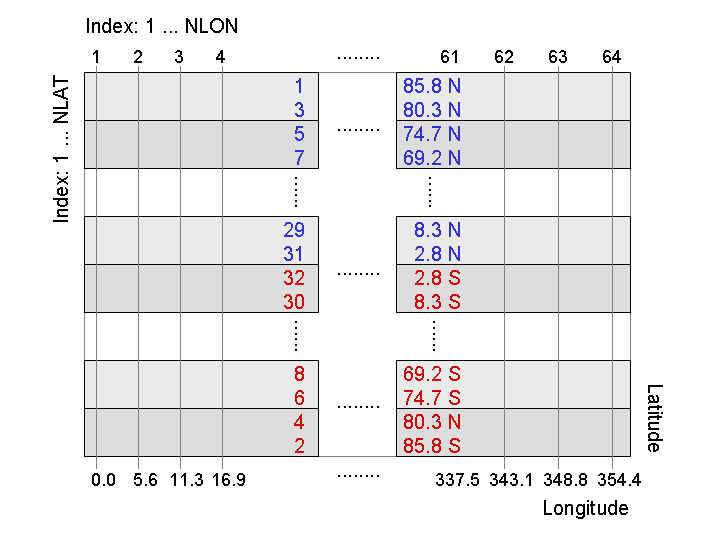
\includegraphics[width=14cm]{Pics/PUMA_alternate_grid_geogr.png}
   \caption[]{PUMA T21 horizontal grid sorted from North to South}
   \label{pumat21lgrid}
\end{figure}


